\documentclass[]{beamer}
\usepackage{etex}
\usetheme[pageofpages=of,% String used between the current page and the
                         % total page count.
          bullet=circle,% Use circles instead of squares for bullets.
          titleline=true,% Show a line below the frame title.
          alternativetitlepage=true,% Use the fancy title page.
          ]{Torino}
\usepackage{soul}
\usepackage{hyperref}

\usepackage{mathtools}
\usepackage{listings}
\usepackage{tikz}
\usepackage{placeins}
\usepackage{lscape}
\usepackage{float}
\usepackage{graphicx}
\usepackage[usenames,dvipsnames]{xcolor}
\usepackage[breakable, skins]{tcolorbox}
\graphicspath{{images/}}

\usepackage{flafter}
\usepackage{pgfplots}
\DeclareFontShape{OT1}{cmtt}{bx}{n}{<5><6><7><8><9><10><10.95><12><14.4><17.28><20.74><24.88>cmttb10}{}
\usetikzlibrary{arrows,automata,shapes}
\usetikzlibrary{positioning}
\usetikzlibrary{shapes.geometric}
\usetikzlibrary{shapes.arrows}
\usepackage{caption}
\captionsetup{font={small}}
\definecolor{darkgreen}{rgb}{0.0,0.5,0.0}
\definecolor{darkred}{rgb}{0.65,0.06,0.06}
\definecolor{mygrey}{rgb}{0.24,0.21,0.2}

\setbeamercolor{structure}{fg=darkgreen}

\pgfplotsset{compat=1.3}
\lstset{
alsoletter=->=,
language=[Objective]{Caml},
basicstyle=\small\ttfamily\color{darkgreen},
numberstyle=\color{black},
numbers=left,
frame=tb,
columns=fullflexible,
showstringspaces=false,
morekeywords={let, in, type, of, fun, if, then, else, rec, as, true, false, math, with, when, open, function, for, sig, ->,>>=,=},
keywordstyle=\ttfamily\bfseries
}

\tikzset{
  invisible/.style={opacity=0},
  visible on/.style={alt={#1{}{invisible}}},
  alt/.code args={<#1>#2#3}{%
    \alt<#1>{\pgfkeysalso{#2}}{\pgfkeysalso{#3}} % \pgfkeysalso doesn't change the path
  },
  function/.style={
         rectangle,
         anchor=center,
         rounded corners,
         node distance=6em,
         draw=black, very thick,
         minimum height=2em,
         inner sep=2pt,
         text centered,
         },
   functionH/.style={
         rectangle,
         anchor=center,
         rounded corners,
         node distance=6em,
         draw=black, very thick, fill=darkgreen,
         minimum height=2em,
         inner sep=2pt,
         text centered,
         },
  decision/.style = { 
    diamond, draw=black, very thick, fill=black!5,
    minimum height=1em,
    node distance=7em,
    text width=3em, text badly centered,
    inner sep=1pt, rounded corners 
    }
}
\tikzset{onslide/.code args={<#1>#2}{%
  \only<#1>{\pgfkeysalso{#2}} % \pgfkeysalso doesn't change the path
}}
\tikzset{temporal/.code args={<#1>#2#3#4}{%
  \temporal<#1>{\pgfkeysalso{#2}}{\pgfkeysalso{#3}}{\pgfkeysalso{#4}} % \pgfkeysalso doesn't change the path
}}



\newcommand{\lstinlinewhite}[1] {\lstinline[basicstyle=\small\ttfamily\color{white}]{#1}}


\newcommand{\BigO}{\ensuremath{\mathcal{O}}}

\newcommand{\myhfill}{\hskip0pt plus 1filll}

\setbeamertemplate{footline}
{
  \leavevmode%
  \hbox{%
  \begin{beamercolorbox}[wd=.4\paperwidth,ht=2.25ex,dp=1ex,center]{author in head/foot}%
    \usebeamerfont{author in head/foot}\insertshortauthor
  \end{beamercolorbox}%
  \begin{beamercolorbox}[wd=.6\paperwidth,ht=2.25ex,dp=1ex,center]{title in head/foot}%
    \usebeamerfont{title in head/foot}\insertshorttitle\hspace*{3em}
    \insertframenumber{} / \inserttotalframenumber\hspace*{1ex}
  \end{beamercolorbox}}%
  \vskip0pt%
}

\tcbset{enhanced}

\DeclareRobustCommand{\mybox}[2][gray!20]{%
\begin{tcolorbox}[   %% Adjust the following parameters at will.
        breakable,
        left=0pt,
        right=0pt,
        top=0pt,
        bottom=0pt,
        colback=#1,
        colframe=#1,
        width=\dimexpr\textwidth\relax, 
        enlarge left by=0mm,
        boxsep=5pt,
        arc=0pt,outer arc=0pt,
        ]
        #2
\end{tcolorbox}
}
\newcommand{\quest}[1]{\mybox{#1}}


\author{Clemens Brunner}
\institute{clemens.brunner@student.uibk.ac.at}
\title{LFSR}
\subtitle{Demonstration of calculation of the states of a single linear feedback shift register}
\date{\today}

\begin{document}
\begin{frame}[t,plain]
\titlepage
\end{frame}

\section{Introduction}

\begin{frame}[t]{Introduction}
  \quest{
  \alert<3>{\alert<4>{Demonstrate} conceptually} and \alert<4>{by example \alert<3>{how the state of a \alert<2>{single linear feedback shift register (LFSR)} can be calculated with algebra.}} \alert<5>{Derive conclusions for the security of ciphers based on LFSRs}.
  }
  Table of Content:
  \begin{enumerate}
    \item Introduction
    \item<2-> Linear feedback shift register
    \item<3-> Conceptual demonstration: Calculation of states
    \item<4-> Example: Calculation of states
    \item<5-> Security of cipher based on LFSR
    \item<6-> Conclusion
  \end{enumerate}
\end{frame}

\section{Linear feedback shift register}


\begin{frame}[t]{Outline}
\tableofcontents[currentsection]
\end{frame}


\begin{frame}[t]{Linear feedback shift register}
\begin{figure}[ht]
\centering
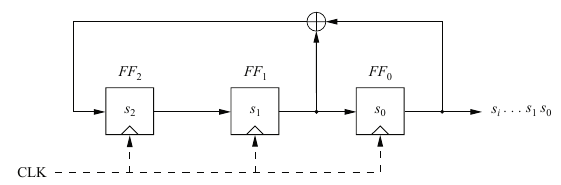
\includegraphics[width=\textwidth]{lfsr_sample.png}
\caption{LFSR of degree 3 with initial values $s_2, s_1, s_0$ [Paar Christof 2009]}
\label{fig:lfsr_sample}
\end{figure}
\begin{itemize}
  \item<2-> Initial state: $(s_2, s_1, s_0) = (1,0,0)$
\end{itemize}
\end{frame}

\begin{frame}[t]{Linear feedback shift register}
\begin{figure}[ht]
\centering
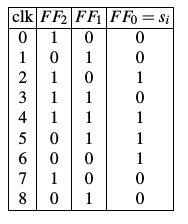
\includegraphics[width=0.3\textwidth]{lfsr_sample_states.png}
\caption{Sequence of states of the LFSR [Paar Christof 2009]}
\label{fig:lfsr_sample_states}
\end{figure}
\end{frame}

\section{Conceptual demonstration: Calculation of states}

\begin{frame}[t]{Outline}
\tableofcontents[currentsection]
\end{frame}


\begin{frame}[t]{Conceptual demonstration}
\begin{figure}[ht]
\centering
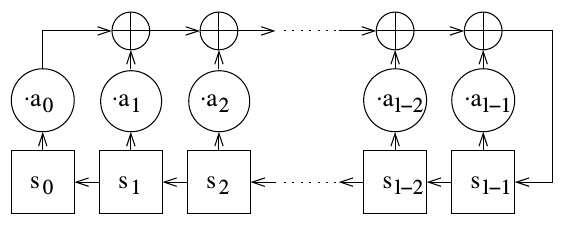
\includegraphics[width=\textwidth]{lfsr.png}
\caption{LFSR [Zenner Erik 2005]}
\label{fig:lfsr}
\end{figure}
\end{frame}

\begin{frame}[t]{Conceptual demonstration}
\begin{itemize}
 \item Feedback vector is unknown it is possible to calculate it using 2l consecutive output bits by solving l linear equations
        \only<3->{\begin{center}
        \[
                \begin{array}{l@{\:=\:}l@{\:+\:}l@{\:+\:}l@{\:+\:}l}
                        s_l     & a_0s_0 & a_1s_1 & \dots & a_{l-1}s_{l-1} \\
                        s_{l+1} & a_0s_1 & a_1s_2 & \dots & a_{l-1}s_{l} \\
                        \hspace{3 mm}\vdots   &\hspace{3 mm} \vdots &\hspace{3 mm} \vdots &\hspace{1.5 mm} \vdots &\hspace{4 mm} \vdots\\
                        s_{2l-1} & a_0s_{l-1}  & a_1s_l  & \dots  & a_{l-1}s_{2l-2} \\
                \end{array}
        \]
        \end{center}
        }
        \only<1-2>{
        \begin{figure}[ht]
        \centering
        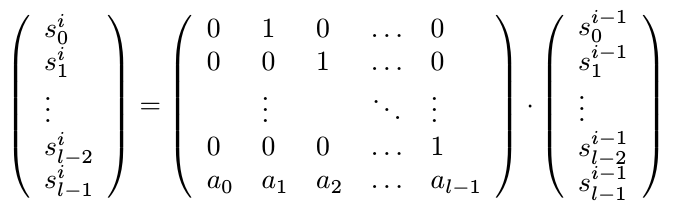
\includegraphics[width=0.6\textwidth]{linear_recursion.png}
        \end{figure}
      }
      \item<4-> If the feedback vector is known it is possible to calculate all following state with knowing l arbitrary output bits.
\end{itemize}
\end{frame}

\section{Example: Calculation of states}

\begin{frame}[t]{Outline}
\tableofcontents[currentsection]
\end{frame}

\begin{frame}[t]{Example: Calculation of states}
\begin{figure}[ht]
\centering
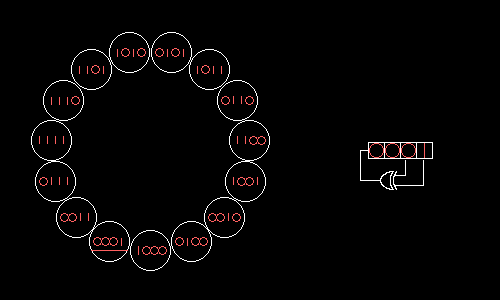
\includegraphics[width=0.7\textwidth]{example_lfsr.png}
\caption{A 4-bit Fibonacci LFSR [Wikipedia]}
\label{fig:example}
\end{figure}

\begin{itemize}
  \item<2-> 2l output-bits: $s_0,s_1,\dots,s_{7}$ are $10001001$
\end{itemize}
\end{frame}

\begin{frame}[t]{Example: Calculation of states}
\begin{itemize}
\item<1-> 2l output-bits: $s_0,s_1,\dots,s_{7}$ are $10001001$ 
\item<1->
        \[
                \begin{array}{l@{\:=\:}l@{\:+\:}l@{\:+\:}l@{\:+\:}l}
                        s_4 & a_0s_0 & a_1s_1  & a_2s_2 & a_3s_3 \\
                        s_5 & a_0s_1 & a_1s_2  & a_2s_3 & a_3s_4 \\
                        s_6 & a_0s_2 & a_1s_3  & a_2s_4 & a_3s_5 \\
                        s_7 & a_0s_3 & a_1s_4  & a_2s_5 & a_3s_6 \\
                \end{array}
        \]
   
\item<2->
        \[
                \begin{array}{l@{\:=\:}l@{\:+\:}l@{\:+\:}l@{\:+\:}l}
                        1 & a_01 & a_10  & a_20 & a_30\\
                        0 & a_00 & a_10  & a_20 & a_31 \\
                        0 & a_00 & a_10  & a_21 & a_30 \\
                        1 & a_00 & a_11  & a_20 & a_30 \\
                \end{array}
        \]

\end{itemize}
\end{frame}


\begin{frame}[t]{Example: Calculation of states}
\begin{table}[h]
\centering
\begin{tabular}{ccc}
$\left[ {\begin{array}{cccc|c}
1 & 0 &  0 & 0 & \mathbf{1} \\
0 & 0 &  0 & 1 & \mathbf{0} \\
0 & 0 &  1 & 0 & \mathbf{0} \\
0 & 1 &  0 & 0 & \mathbf{1} 
 \end{array} } \right]$

& \underrightarrow{\textrm{Switch row 2 and 4}}  &


$\left[ {\begin{array}{cccc|c}
1 & 0 &  0 & 0 & \mathbf{1} \\
0 & 1 &  0 & 0 & \mathbf{1} \\
0 & 0 &  1 & 0 & \mathbf{0} \\
0 & 0 &  0 & 1 & \mathbf{0} 
 \end{array} } \right]$
 \\

\end{tabular}
\end{table}
\begin{itemize}

\item $a_0=1$, $a_1=1$, $a_2=0$, $a_3=0$
\end{itemize}
\end{frame}

\begin{frame}[t]{Example: Calculation of states}
\begin{itemize}
  \item Feedback vector: \:$a_3=0$, $a_2=0$,  $a_1=1$, $a_0=1$
  \item l initial sequence: $s_3=0$, $s_2=0$, $s_1=0$, $\:s_2=1$
  \item Formula: $s_n = s_{n-1}a_3 + s_{n-2}a_2 + s_{n-3}a_1 + s_{n-4}a_0$
  \item Calculated output: \onslide<4->{1}\onslide<6->{0}\onslide<8->{0}\onslide<10->{1}\onslide<12->{1}\onslide<14->{0}\onslide<16->{1}\onslide<17->{\dots}
  \only<3,4>{\item $s_4 = \mathbf{0}*0 + \mathbf{0}*0 + \mathbf{0}*1 + \mathbf{1}*1$}
  \only<5,6>{\item   $s_5 = \mathbf{1}*0 + \mathbf{0}*0 + \mathbf{0}*1 + \mathbf{0}*1$}
  \only<7,8>{\item   $s_6 = \mathbf{0}*0 + \mathbf{1}*0 + \mathbf{0}*1 + \mathbf{0}*1$}
  \only<9,10>{\item   $s_7 = \mathbf{0}*0 + \mathbf{0}*0 + \mathbf{1}*1 + \mathbf{0}*1$}
  \only<11,12>{\item  $s_8 = \mathbf{1}*0 + \mathbf{0}*0 + \mathbf{0}*1 + \mathbf{1}*1$}
  \only<13,14>{\item  $s_9 = \mathbf{1}*0 + \mathbf{1}*0 + \mathbf{0}*1 + \mathbf{0}*1$}
  \only<15->{\item  $s_{10} = \mathbf{0}*0 + \mathbf{1}*0 + \mathbf{1}*1 + \mathbf{0}*1$}
\end{itemize}

\end{frame}

\begin{frame}[t]{Example: Calculation of states}
\begin{figure}[ht]
\centering
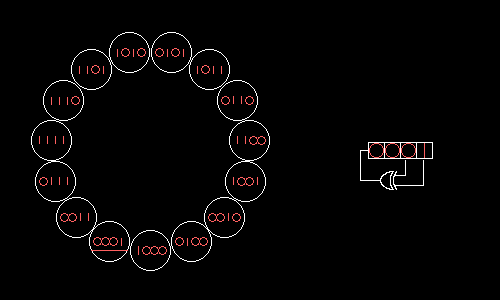
\includegraphics[width=0.7\textwidth]{example_lfsr.png}
\caption{A 4-bit Fibonacci LFSR [Wikipedia]}
\end{figure}
\end{frame}

\section{Security of cipher based on LFSR}
\begin{frame}[t]{Outline}
\tableofcontents[currentsection]
\end{frame}

\begin{frame}[t]{Security of cipher based on LFSR}
\begin{itemize}
  \only<1>{\item Single LFSRs are insecure}
  \only<2->{\item\st{Single} LFSRs are secure}
  \onslide<3->{
 \begin{figure}[ht]
\centering
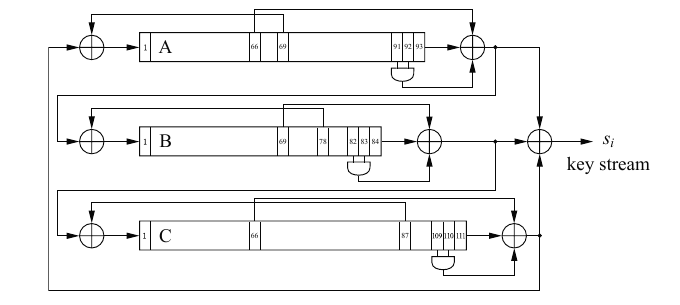
\includegraphics[width=0.8\textwidth]{trivium.png}
\caption{Trivium [Paar Christof 2009]}
\label{fig:trivium}
\end{figure}
}
\end{itemize}
\end{frame}


\section{Summary}
\begin{frame}[t]{Conclusion}
   \quest{
  \alert<3>{\alert<4>{Demonstrate} conceptually} and \alert<4>{by example \alert<3>{how the state of a \alert<2>{single linear feedback shift register (LFSR)} can be calculated with algebra.}} \alert<5>{Derive conclusions for the security of ciphers based on LFSRs}.
  }
\end{frame}

\bibliography{biblio}{}
\bibliographystyle{plain}

\begin{frame}[t]{End}
  \begin{center} \LARGE{Any Questions?} \end{center}
  \only<>{
  \cite{Zenner-Erik}
  \cite{Paar-Christof}}
\end{frame}


\end{document}

